%%%%%%%%%%%%%%%%%%%%%%%%%%%%%%%%%%%%%%%%%%%%%%%%%%%%%%%%%%%
%%%%%%%%%%%%%%%%%%%%%%%%%%%%%%%%%%%%%%%%%%%%%%%%%%%%%%%%%%%
\subsection{EMMA}

%%%%%%%%%%%%%%%%%%%%%%%%%%%%%%%%%%%%%%%%%%%%%%%%%%%%%%%%%%%%%%%%%%%%%%%%%%%%%%%%%%%%%%%%5
%\subsubsection{all samples}
A total of 30 recipes (see \ref{sec:app-emma}) have been investigated in 
five iterations of the algorithm ($t = 0, \dots, 4$). 
%The best recipe identified by the EMMA algorithm is as follows: 
The best recipes for each generation can be seen in table \ref{tab:emma-Gb}. 
The calcination heating $v_{cal}$ rate has been predicted perfectly 
\td{even though $v_{cal}$ doesn't appear in the prediction function, how is this possible?}
The number of layers $\lambda$ on the other hand was predicted poorly 
even though the conversion factor wsa 1 and the prediction function dependent on $\lambda$. 

%%%%%%%%%%%%%%%%%%%%%%%%%%%%%%%%%%%%%%%%%%%%%%%%%%%%%%%%%%%%%%%%%%%%%%%%%%%%%%%%%%%%%%%%5
\subsubsection{how did evolve over time?}

\begin{figure}[htb]
    \centering
    \begin{subfigure}{.45\textwidth}
        \centering
        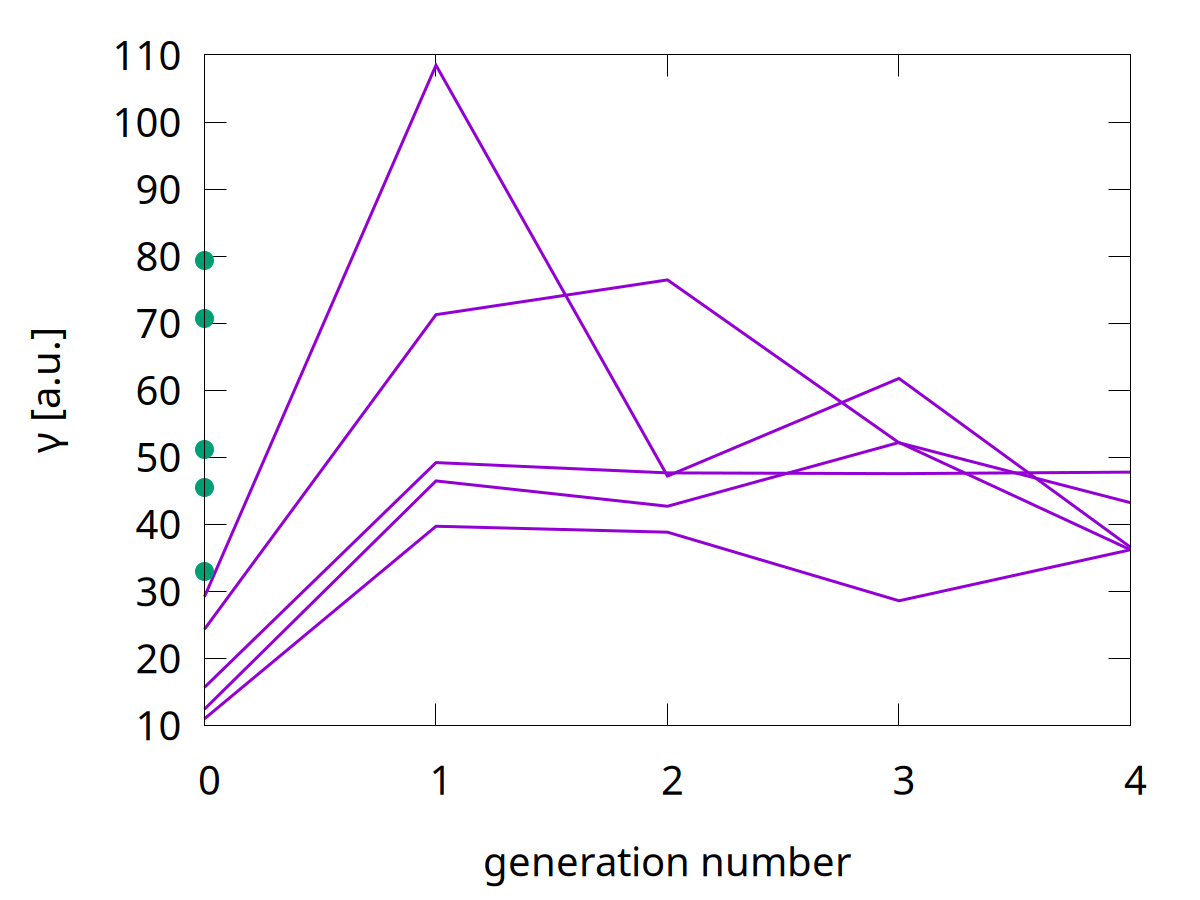
\includegraphics[width=.8\textwidth]{Pics/stats/gen-G.png}
        \caption{emma G gen } \label{fig:emma-G-gen}
    \end{subfigure}
    \begin{subfigure}{.45\textwidth}
        \centering
        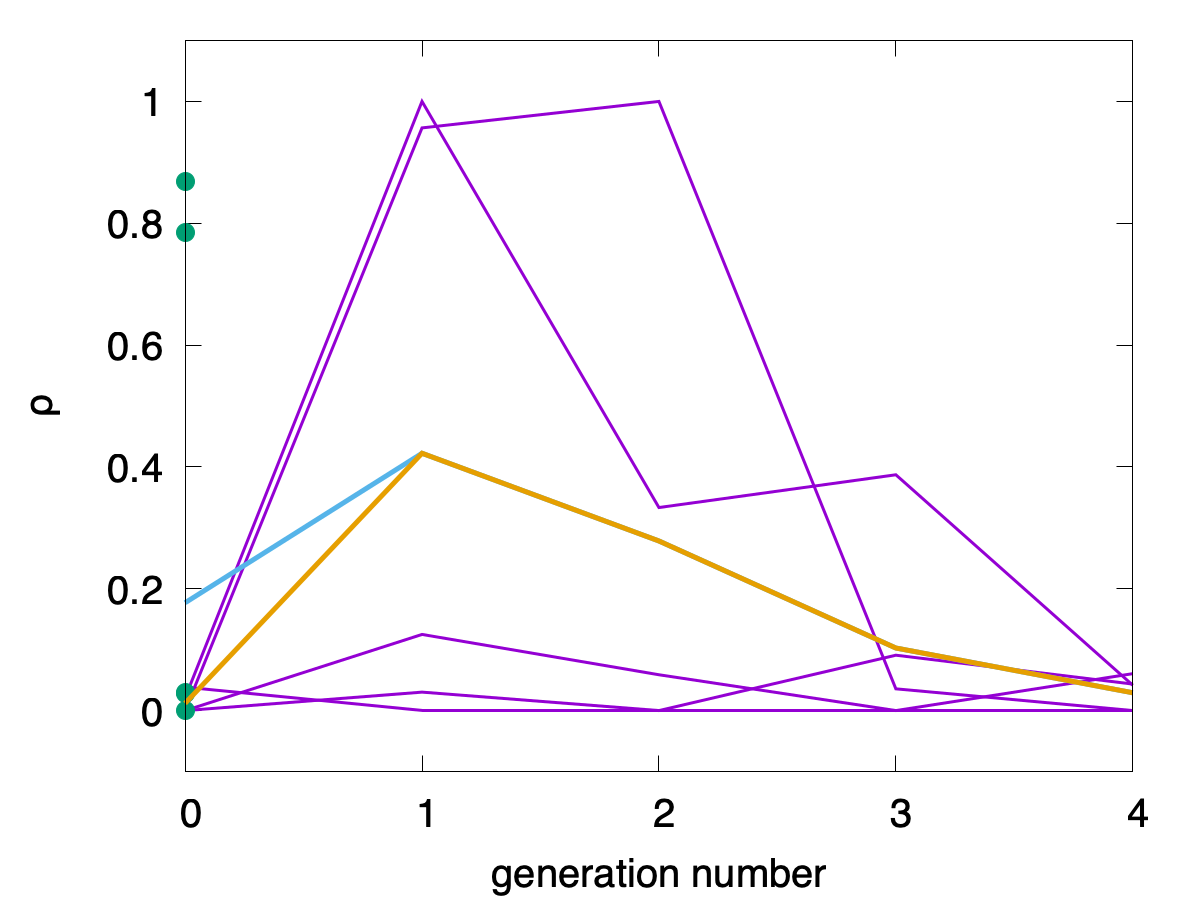
\includegraphics[width=.8\textwidth]{Pics/stats/gen-phd.png}
        \caption{emma phd gen} \label{fig:emma-phd-gen}
    \end{subfigure}
    \caption{emma gen} \label{fig:emma-gen}
\end{figure}

In figure \ref{fig:emma-gen} we can see the two main optimizables at each generation
for each particle.
It shows a clear trend which indicates that the optimization worked even though 
the predicted function and the chosen samples where not exactly as expected. 
This might be due to the high error of samples. 


\begin{table}[htb]
	\centering
    \caption{Global best per generation}
	\label{tab:emma-Gb}
	\begin{tabular}{cccccccc}
        \hline\hline
    generation  &enr &conc &layr &vDOC &TDOC &vCal &TCal\\
        \hline
     1   &1       &2    &4   &10   &40  &120  &300\\
     2   &5       &2    &6   &10   &40  &120  &300\\
     3   &2947    &4    &6   &16   &80 &1080  &300\\
     4   &2405    &2    &6   &10   &40 &1080  &300\\
     5   &13      &2   &10   &10   &40  &120  &300\\
    \hline\hline
	\end{tabular}
\begin{tabular}{cccccc}
    \hline\hline
enr     &1st gen     &2nd gen        &3rd gen        &4th gen        &5th gen\\
    \hline
1       &1.214185    &       &       &       &38.7962       \\
5       &       &4.196626       &       &       &25.47335       \\
2947    &       &       &10.9594    &       &10.9594       \\
2405    &       &       &       &20.04962   &25.47335       \\
13      &       &       &       &       &24.87178   \\
    \hline\hline
\end{tabular}
\end{table}

%\iffalse
%\fi

\iffalse
\begin{figure}
\centering
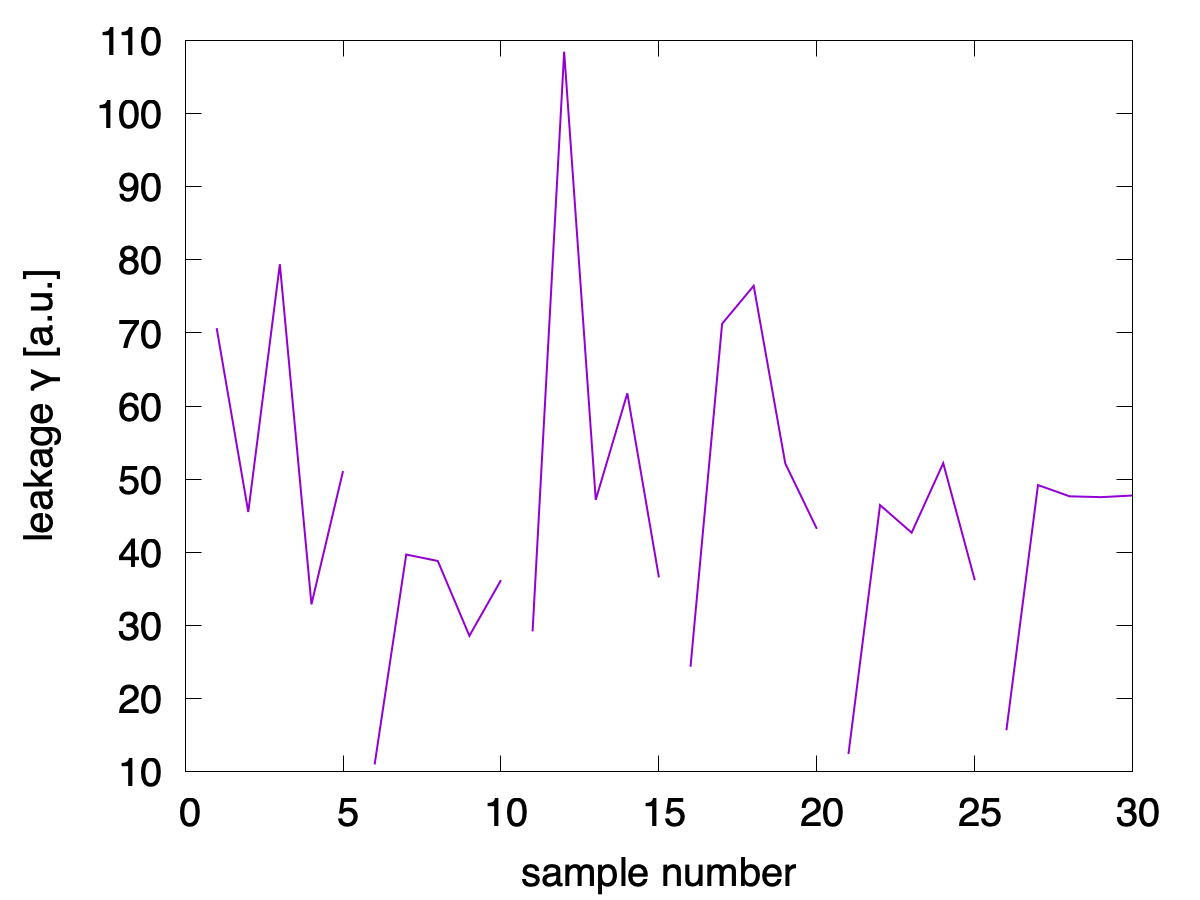
\includegraphics[width=.6\textwidth]{Pics/stats/G-t.png}
    \caption{conductivity G [a.u.] against sample number (is this even correct?)}
    \label{fig:G-t}
\end{figure}

\td{TODO: check if the sorted correctly? Make generation graph with boxplot }
\td{TODO: visualize} how the population moved across the space (with parallel coordinates? or see page 121)
\url{https://stackoverflow.com/questions/30228281/gnuplot-parallel-coordinates-axes-plot-key-annotation}
\fi

%%%%%%%%%%%%%%%%%%%%%%%%%%%%%%%%%%%%%%%%%%%%%%%%%%%%%%%%%%%%%%%%%%%%%%%%%%%%%%%%%%%%%%%%5
\subsubsection{what is best}
\begin{align}
    G &=      -19 + 0.28 * TCal  - 0.022 * layr*TCal  +  0.16 * h(layr-6)*TDOC \\
    \rho &=  -0.87 + 0.0047 * TCal  - 0.00036 * layr*TCal  +  0.0024 * h(layr-6)*TDOC \\
    \lambda &=  6.8 - 0.014 * TCal  + 0.0018 * layr*TCal  + 0.0060 * h(layr-6)*TDOC \\
    v_{cal} &= 29 - 0.052 * TCal  + 0.0011 * layr*TCal  -  0.011 * h(layr-6)*TDOC 
    \label{eq:emma}
\end{align}
%what was the best result? For each particle there is best and global best. 

%%%%%%%%%%%%%%%%%%%%%%%%%%%%%%%%%%%%%%%%%%%%%%%%%%%%%%%%%%%%%%%%%%%%%%%%%%%%%%%%%%%%%%%%5
\subsubsection{how did model selection influence results}
The heating rate of the calcination process $v_{cal}$ and the number of layers $\lambda$ were included as dependent variable with the objective to maximize with a relative weight of 0.05.
The idea was to maximize $v_{cal}$ and minimize $\lambda$ in order to minimize the process time. 
Another thought behind including $v_{cal}$ and $\lambda$ was to test if the alogrithm would correctly predict those. 
Two major flaws behind this flaws became obvious with time: 
(1) The algorithm would be influenced by those values to choose samples, which potenitally optimize $v_{cal}$ and/or $\lambda$ but not $G$ or $\rho$. 
Neben making the problem unnoetiger weise more complicate, important time (around 10\% of the samples) could have been replaced with more insighful samples. 
(2) The true function for predicting $v_{cal}$ and $\lambda$ are $v_cal*60$ ($C/h$ instead of $C/min$) and $\lambda$, respectively. 
The algorithm will tend to include thos values into the prediction function for all dependent variables and possibly exclude others which have more influence on $G$ and $\rho$ (see \ref{eq:emma}).
\begin{itemize}
    \item MARS chooses same set from independent variables for predicting all dependent variables. 
    \item flaws of MARS: all functions are dependent on same indep vars
    \item Every output var is independent of each other, so $v_{cal}$ can act as test 
heating rate was one of the dependent variables with the intention of minimizing the variable. 
It can also be used as test to see how well the EMMA performes (or rather, more precisely MARS)
It doesn't influence the fit for the other splines, but it influences the choice of samples therefore it might have slowed down the process
Overall there were too many variables involved for such a small dataset
        that means that adding dependent variables influences \td{previous variables}
\end{itemize}

\td{look at emma papers}
